%%%%%%%%%%%%%%%%%%%%%%%%%%%%%%%%%%%%%%%%%%%%%%%%%
%%%%%%%%%%%%%%%%%%%%%%%%%%%%%%%%%%%%%%%%%%%%%%%%%

\chapter[L'HCERES]{L'HCERES} \label{HCERES}

\index{Haut conseil de l'\'evaluation de la recherche et de l'enseignement sup\'erieur (HCERES)}

Cr\'e\'e par la loi no. 2013-660 du 22 juillet 2013 relative \`a l'Enseignement Sup\'erieur et \`a la Recherche (ESR), 
le Haut Conseil de l'\'evaluation de la recherche et de l'enseignement sup\'erieur (HCERES) se substitue 
\`a l'Agence d'\'evaluation de la recherche et de l'enseignement sup\'erieur (AERES).

Ce conseil est la {\em seule} autorit\'e administrative fran\c caise
charg\'ee de l'\'evaluation de l'enseignement sup\'erieur et de la recherche publics.
L'HCERES a pour vocation de rassembler sous un m\^eme toit les ex-MSTP, ex-CNE
et ex-CNER\footnote{%
MSTP~: Mission scientifique, technique et p\'edagogique~;
CNE~: Comit\'e national d'\'evaluation
des \'etablissements publics \`a caract\`ere scientifique, culturel et
professionnel~;
CNER~: Comit\'e national d'\'evaluation de la recherche},
et d'assurer les missions d'\'evaluation des EPSCP (donc les universit\'es), des EPST (donc le CNRS, INRIA...),
leur recherche (donc les laboratoires) et leur formation.
On rappelle que les équipes Inria ne sont pas évaluées par l'HCERES, c'est l'établissemnt qui est évalué. 
Les équipes sont évaluées depuis des années suivant une procédure propre à Inria (cf chap. \ref{INRIA}). 

Toutes les informations de ce chapitre sont tir\'ees du site de l'agence: \lien{www.hceres.fr}


%%%%%%%%%%%%%%%%%%%%%%%%%%%%%%%%%%%%%%%%%%%
\section{Statut, missions et organisation}

Le Haut Conseil de l'\'evaluation de la recherche et de l'enseignement sup\'erieur (HCERES) est une autorit\'e administrative ind\'ependante. 
Pour l'exercice de ses missions, le Haut Conseil s'inspire des meilleures pratiques internationales. Il fonde son action, en ce qui concerne les crit\`eres d'\'evaluation, sur les principes d'objectivit\'e, 
de transparence et d'\'egalit\'e de traitement entre les structures examin\'ees et, en ce qui concerne le choix des personnes charg\'ees de l'\'evaluation, sur les principes d'expertise scientifique au meilleur niveau international, 
de neutralit\'e et d'\'equilibre dans la repr\'esentation des th\'ematiques et des opinions. Il veille \`a la pr\'evention des conflits d'int\'er\^ets dans la constitution des comit\'es d'expert$\cdot$es charg\'e$\cdot$es de conduire les \'evaluations. 
Il peut conduire directement des \'evaluations ou s'assurer de la qualit\'e des \'evaluations r\'ealis\'ees par d'autres instances en validant les proc\'edures retenues. Il met en mesure les structures et \'etablissements qu'il \'evalue directement de pr\'esenter, 
\`a leur demande, des observations tout au long et \`a l'issue de la proc\'edure d'\'evaluation.

Le HCERES est charg\'e:
\begin{itemize}
\item d'\'evaluer les \'etablissements d'enseignement sup\'erieur et leurs regroupements, les organismes de recherche, les fondations de coop\'eration scientifique et l'Agence nationale de la recherche ou, le cas \'ech\'eant, de s'assurer de la qualit\'e des \'evaluations conduites par d'autres instances ;
\item d'\'evaluer les unit\'es de recherche \`a la demande de l'\'etablissement dont elles rel\`event, en l'absence de validation des proc\'edures d'\'evaluation ou en l'absence de d\'ecision de l'\'etablissement dont rel\`event ces unit\'es de recourir \`a une autre instance ou, le cas \'ech\'eant, 
de valider les proc\'edures d'\'evaluation des unit\'es de recherche par d'autres instances.
\end{itemize}
Le HCERES \textbf{ne fait pas d'évaluation individuelle}. 

\quad

Lorsqu'une unit\'e rel\`eve de plusieurs \'etablissements, il n'est proc\'ed\'e qu'\`a une seule \'evaluation. 
Lorsque les \'etablissements d\'ecident conjointement de recourir \`a une autre instance, le Haut Conseil valide les proc\'edures d'\'evaluation mises en \oe uvre par cette instance. Dans le cas contraire, le Haut Conseil \'evalue l'unit\'e de recherche,
\begin{itemize}
\item en \'evaluant les formations et dipl\^omes des \'etablissements d'enseignement sup\'erieur ou, le cas \'ech\'eant, 
en validant les proc\'edures d'\'evaluation r\'ealis\'ees par d'autres instances.
\item en s'assurant de la prise en compte, dans les \'evaluations des personnels de l'enseignement sup\'erieur et de la recherche, de l'ensemble des missions qui leur sont assign\'ees par la loi et leurs statuts particuliers ;
\item en s'assurant de la valorisation des activit\'es de diffusion de la culture scientifique, technique et industrielle dans la carri\`ere des personnels de l'enseignement sup\'erieur et de la recherche ;
\item en \'evaluant a posteriori les programmes d'investissement et les structures de droit priv\'e recevant des fonds publics destin\'es \`a la recherche ou \`a l'enseignement sup\'erieur. 
\end{itemize}
Dans le cadre de programmes de coop\'eration europ\'eens ou internationaux ou \`a la demande des autorit\'es comp\'etentes, le HCERES peut participer \`a l'\'evaluation d'organismes \'etrangers ou internationaux de recherche et d'enseignement sup\'erieur.

Le Haut Conseil comporte \'egalement un Observatoire des Sciences et Techniques (OST) charg\'e de conduire des \'etudes et analyses strat\'egiques. 

On notera que les évaluations se font \textit{par vagues}: A, B, C, D ou E.
Le Haut Conseil a ainsi défini un cycle de campagnes d'évaluation calquées sur cette répartition \textit{par vagues}. 
(ex.~: Vague A de contractualisation 2016-2020 \'evalu\'ee en 2014-2015). 
Tous les ans, il évalue les établissements d'une même \textit{vague}.
On trouve sur le site officiel, \href{http://www.hceres.fr/PUBLICATIONS/Rapports-d-evaluation/Listes-alphabetiques/Liste-des-etablissements-evalues-par-academie}{classé par établissements},
les rapports des précédentes évaluations et à quelle vague appartient un établissement.


%L'HCERES est une autorit\'e administrative ind\'ependante charg\'ee
%d'\'evaluer
%les \'etablissements et organismes de recherche (et
%d'enseignement sup\'erieur, le cas \'ech\'eant), ainsi que leurs
%activit\'es de recherche. Elle est \'egalement charg\'ee de
%l'\'evaluation de l'ANR et des formations et dipl\^omes de
%l'enseignement sup\'erieur. En ce qui concerne l'\'evaluation des
%{\em individus}, l'HCERES n'est charg\'ee que de valider les
%proc\'edures men\'ees soit par le CNU (dans les universit\'es), soit
%par le Comit\'e National (pour les chercheurs CNRS) ; nous renvoyons
%pour cela aux sections suivantes. Il est \`a noter qu'INRIA \'evalue ses
%\'equipes-projets, mais ne pratique pas d'\'evaluation individuelle,
%sauf lors d'une mutation et/ou d'une promotion, voir les sections \ref{CE-INRIA}
%et \ref{sec. projets INRIA}.
%
%\medskip
%
%L'HCERES est organis\'ee en trois sections correspondant \`a ses principales missions~:
%
%\begin{itemize}
%
%\item La {\em section des \'etablissements} est comp\'etente, d'une part, pour
%\'evaluer les \'etablissements et organismes li\'es \`a la recherche et,
%d'autre part, pour valider les proc\'edures d'\'evaluation de leurs
%personnels, et pr\'eparer un avis
%sur les conditions dans lesquelles elles sont mises en \oe uvre.
%
%\item La {\em section des unit\'es de recherche} est comp\'etente pour l'\'evaluation des
%activit\'es des unit\'es de recherche des \'etablissements et organismes
%li\'es \`a la recherche. Elle conduit l'\'evaluation soit directement,
%soit en s'appuyant sur les \'etablissements et organismes selon
%des proc\'edures qu'elle a valid\'ees.
%
%\item La {\em section des formations} est comp\'etente pour l'\'evaluation des
%formations et des dipl\^omes (licence, master).
%\end{itemize}
%
%\medskip
%
%Chaque {section} est dirig\'ee par un directeur nomm\'e pour un mandat de quatre ans renouvelable
% par le conseil de l'agence sur proposition du pr\'esident de l'agence. Aux c\^ot\'es de ces sections, si\`ege
% ledit {conseil}, compos\'e de 25 membres renouvel\'es par moiti\'e tous les deux ans, nomm\'es par
% diff\'erentes instances (minist\`ere, organismes de recherche, CNU, comit\'e national, parlement). Chaque
% \'evaluation est conduite par un {comit\'e d'\'evaluation}, dont les membres sont choisis par le pr\'esident
% de la section concern\'ee, apr\`es avis et propositions du conseil, des pr\'esidents ou directeurs des
%\'etablissement d'ESR, des chefs d'instances d'\'evaluation nationale.\\

\bigskip

Le HCERES est administr\'e par un conseil garant de la qualit\'e de ses travaux. Le conseil arr\^ete le programme annuel d'\'evaluation du Haut Conseil. Il d\'efinit les mesures propres \`a garantir la qualit\'e, la transparence et la publicit\'e des proc\'edures d'\'evaluation. Son pr\'esident ou sa Pr\'esidente, nomm\'e$\cdot$e parmi ses membres, dirige le Haut Conseil et a autorit\'e sur ses personnels. Le conseil est compos\'e de trente membres nomm\'es par d\'ecret pour une dur\'ee de quatre ans, renouvelable une fois.

Le conseil comprend :
\begin{itemize}
\item Neuf membres ayant la qualit\'e de chercheur$\cdot$se, d'ing\'enieur$\cdot$e ou d'enseignant$\cdot$e-chercheur$\cdot$se, nomm\'e$\cdot$es sur proposition des instances d'\'evaluation comp\'etentes en mati\`ere d'enseignement sup\'erieur et de recherche parmi leurs membres \'elu$\cdot$es, dont au moins trois sur proposition de l'instance nationale mentionn\'ee 
\`a l'article L. 952-6 du code de l'\'education et au moins trois sur proposition des instances d'\'evaluation mentionn\'ees \`a l'article L. 321-2 du pr\'esent code ;
\item Huit membres ayant la qualit\'e de chercheur$\cdot$se, d'ing\'enieur$\cdot$e ou d'enseignant$\cdot$e-chercheur$\cdot$se, dont trois sur proposition des pr\'esident$\cdot$es ou directeur$\cdot$trices d'organismes de recherche et trois sur proposition des conf\'erences des chefs d'\'etablissements mentionn\'ees \`a l'article L. 233-1 du code de l'\'education ;
\item Deux membres repr\'esentant les \'etudiant$\cdot$es, sur proposition des associations d'\'etudiant$\cdot$es en fonction du nombre de voix obtenues par ces associations lors de l'\'election des repr\'esentants des \'etudiant$\cdot$es au Conseil national de l'enseignement sup\'erieur et de la recherche ;
\item Neuf personnalit\'es qualifi\'ees, fran\c caises et \'etrang\`eres, dont au moins trois issues du secteur de la recherche priv\'ee et trois appartenant \`a des agences d'accr\'editation ou d'\'evaluation \'etrang\`eres ;
\item Un$\cdot$e d\'eput\'e$\cdot$e et un$\cdot$e s\'enateur$\cdot$trice d\'esign\'e$\cdot$es par la commission permanente comp\'etente en mati\`ere d'enseignement sup\'erieur et de recherche de chaque assembl\'ee.
\end{itemize}
 


 


%Voici l'organigramme qu'on peut trouver sur le site de l'HCERES :
%
%\begin{center}
%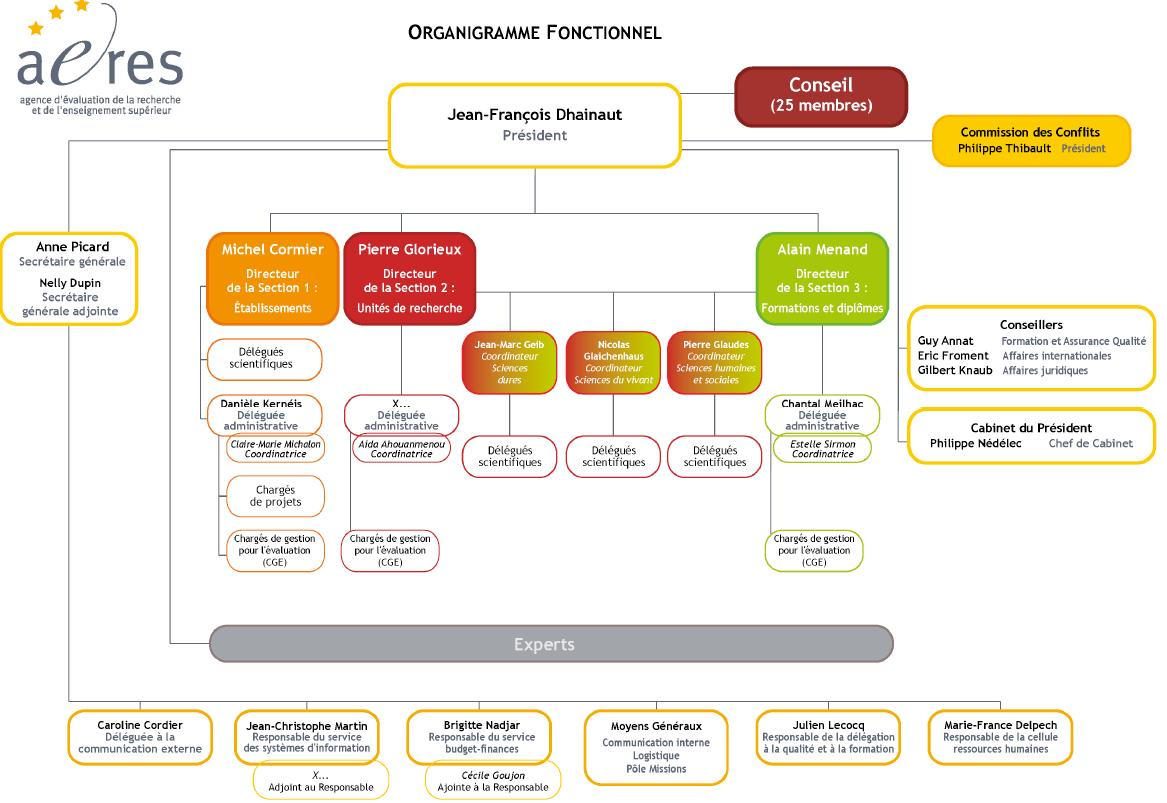
\includegraphics[width=12cm]{organigramme_aeres.jpg}
%\end{center}
%
%Il est \`a noter que le point le plus critiqu\'e par la communaut\'e scientifique sur le fonctionnement de
% l'AERES est le fait que \textit{tous} les membres soient \textit{nomm\'es}, ce qui peut \^etre
%consid\'er\'e en contradiction avec l'objectif d'ind\'ependance affich\'e par la loi.\\
%
%Le d\'ecret relatif \`a la mise en place de l'agence est disponible sur
%le site du Journal Officiel.\\
%\lien{www.legifrance.gouv.fr/WAspad/UnTexteDeJorf?numjo=MENX0600140D}\\



\section{Les crit\`eres d'\'evaluation}

Les crit\`eres d'\'evaluation des \'etablissements ne sont pas pr\'ecis\'es par les textes
instaurant l'HCERES, et sont donc laiss\'es \`a l'appr\'eciation des comit\'es d'\'evaluation
 (\`a l'exception de la valorisation des recherches, explicitement cit\'ee par la loi).



\section{L'\'evaluation des laboratoires}
\index{Evaluation ! des laboratoires}

La section des unit\'es r\'ealise plus de 700 \'evaluations par an
(chaque unit\'e \'etant \'evalu\'ee tous les cinq ans) sur la base d'un dossier scientifique
remis par l'unit\'e et de visites sur site par un comit\'e d'experts.
Il s'agit d'une \'evaluation transparente et contradictoire,
ax\'ee sur un rapport d'expertise et une notation.
Les rapports d'\'evaluation sont publics et accessibles sur le
web de l'agence~:\\
 \lien{www.hceres.fr/}.\\

Noter qu'on
trouve \'egalement sur ce site les grilles d'\'evaluation qui seront
remplies par les expert$\cdot$es, ce qui permet de se faire une id\'ee des
crit\`eres d'\'evaluation~: outre un profil quantitatif (indiquant
notamment la taille des \'equipes, le nombre de publiant$\cdot$es ou le
nombre de th\`eses en cours et soutenues), y figure \'egalement un
profil qualitatif dans lequel apparaissent l'originalit\'e et
l'int\'er\^et des recherches, le niveau et la notori\'et\'e des
travaux, {\em etc}.

En pratique, lorsque son établissement d'appartenance est évalué, le laboratoire
doit constituer un dossier, qui est sous la responsabilité de la directrice ou du directeur du laboratoire.
Ce dossier contient un rapport
d'activit\'e global du laboratoire, la liste des publications pendant
la p\'eriode de contractualisation finissante, le programme de
recherche pour les cinq ann\'ees \`a venir, \`a l'\'echelle du
laboratoire, et les ressources financi\`eres demand\'ees
pour mener \`a bien ce programme de recherche.


\section{Accr\'editation des \'etablissements d'enseignement sup\'erieur}
\index{Accr\'editation}
\index{Conseil national de l'enseignement sup\'erieur et de la recherche (CNESER)}

Depuis la loi ESR cit\'ee ci-dessus, les \'etablissements ne demandent plus au minist\`ere l'habilitation des formations, 
mais demandent l'accr\'editation pour l'ensemble de leurs formations. Il leur revient alors de s'assurer que les formations respectent 
le cadre national d\'efini par le CNESER (cf. section \ref{CNESER} du chapitre sur le Ministère), 
et de s'assurer qu'ils assurent la qualit\'e  de la formation en l'adossant aux activit\'es de recherche, et en suivant les \'etudiant$\cdot$es dans leurs parcours. 

Aussi sur la base de l'évaluation HCERES, la DGESIP (cf \ref{DGESIP}) du ministère décide de l'accr\'editation pour la dur\'ee de cinq ann\'ees.

\href{https://www.legifrance.gouv.fr/affichTexte.do?cidTexte=JORFTEXT000028543620&categorieLien=id}{Arrêté du 22 janvier 2014 fixant les modalités d'accréditation d'établissements d'enseignement supérieur}

